%!TeX spellcheck = en-US
%!TEX root = ../hw3_report.tex
\subsection*{(a)}

The matrix $A$ is diagonalizable with the  eigendecomposition $A = QDQ^{-1}$, where $D$ is a diagonal matrix. For such structures it holds that $\sin(A) = Q\sin(D)Q^{-1}$. Thus we can validate the result for the Schur-Parlett method, which is
\begin{equation}
  \sin(A) = \sin\left(\begin{bmatrix}
    1 & 4 & 4\\
    3 & -1 & 3\\
    -1 & 4 & 4
  \end{bmatrix}\right) \approx  \begin{bmatrix}
  0.846192 & 0.0655435 & -0.187806\\
 0.33476  & 0.385017  & -0.141244\\
-0.190921 & 0.192478  &  0.848269
  \end{bmatrix}.
\end{equation}
which in norm differs $4.28e-16$ from $Q\sin(D)Q^{-1}$.


%\lstinputlisting{"/Users/Fryklund/Documents/julia/SF3580/src/schur_parlett.jl"}

%\lstinputlisting{"/../../../src/schur_parlett.jl"}

\subsection*{(b) \& (c)}

It is clear from Figure \ref{fig:task5bc} that the number of flops required for Schur--Parlett is not discernibly affected by $N$, at leat for $N \in {10,50,100,150,200,250,300}$. This is not suprsining, as often the most computationally demanding part of the Schur--Parlett method, in  is performing the Schur decomposition, which scales like $\mathcal{O}(n^{3})$. Once obtained, the function $f$ is only applied to the diagonal elements, which are scalars.

For the naive appraoch  the number of flops is proportional to $N$. A matrix multiplication is of $\mathcal{O}(n^{3})$, thus performing $N$ matrix gives $\mathcal{O}(Nn^{3})$, which we read from Figure \ref{fig:task5bc}. The black line corresponds to the line $0.08 + 0.07\,N$.


\begin{figure}
\centering
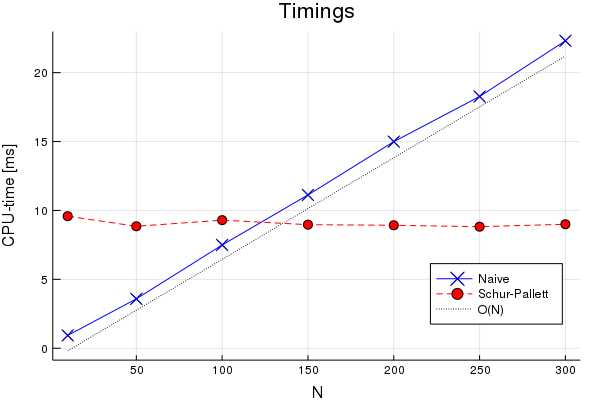
\includegraphics[scale=0.6]{Task5bc}
\caption{Task $5$, (b) \& (c):  CPU--time in milliseconds, as a function of $N$.}
\label{fig:task5bc}
\end{figure}
% \FloatBarrier
